\chapter{Implementation}


\section{Introduction}
After defining the system's architecture and selecting the appropriate methods, the next step is to bring the proposed solution to life through implementation. This chapter presents the practical implementation of our smart wheat monitoring system. It details the tools, technologies, and development environments used throughout the project. We describe the step-by-step construction of each system module, including the wheat disease classification models (binary and multi-class) and insect pest detection model. Furthermore, this chapter outlines the integration and deployment of the trained models within a web-based platform.


\section{Development Environment}
Training the proposed wheat-health models required the use of two distinct compute setups. For the wheat-disease classification task, we initially relied on Google Colab’s free cloud instances due to the absence of a local \gls{abb:gpu}, conducting all training and experimentation in the cloud. Later, for the insect-pest detection task and integration efforts, we utilized a laptop equipped with an NVIDIA RTX 4050 \gls{abb:gpu}, which enabled faster processing and reproducible experiments to be executed locally. More details on the hardware specifications are provided in Table~\ref{tab:hardware-specs}.

\begin{table}[H]
    \caption{Hardware specifications by task}
    \centering
    \resizebox{\textwidth}{!}{%
    \begin{tabular}{|p{4.2cm}|p{5.5cm}|p{5.5cm}|}
        \hline
        \textbf{Component} & \textbf{Wheat-Disease Classification (Google Colab)} & \textbf{Insect-Pest Detection (Local Laptop)} \\
        \hline
        Processor & Intel Xeon or equivalent (shared cloud CPU) & AMD Ryzen 5  \\
        \hline
        GPU & T4 GPU (allocated per session) & NVIDIA GeForce RTX 4050  \\
        \hline
        System Memory & 12 GB & 16 GB  \\
        \hline
        Storage & Limited Google Drive storage & 475 GB SSD \\
        \hline
    \end{tabular}%
    }
    \label{tab:hardware-specs}
\end{table}

A consistent and modular software toolchain was used to support all stages of development, from data preparation to model training and deployment. Full details on the tools, libraries, and configurations are provided in Appendix \ref{app:annexC}.

\section{Implementation of wheat disease  classification modeles}
The development of wheat disease classifiers began with a structured preprocessing pipeline designed to clean, resize, and augment the image data. Two types of models were built: a binary classifier to distinguish between healthy and diseased leaves, and a multi-class classifier to identify specific disease types. 
\subsection{Explaining the Core Training Parameters}
To ensure effective learning and robust model performance, several key training parameters were meticulously configured. These parameters play a critical role in guiding the learning process, enhancing optimization efficiency, and promoting strong generalization to unseen data, ultimately contributing to a more accurate and reliable model.

\begin{itemize}

    \item \textbf{Training/ validation/ test datasets:} are distinct data subsets used at different stages of model development: the training set optimizes model parameters through backpropagation, the validation set tunes hyperparameters and monitors generalization during training, while the test set is used only once and provides an unbiased final evaluation of real-world performance. Together, they ensure robust learning, prevent overfitting, and objectively measure predictive accuracy.

    \item \textbf{Input Shape:} Defines the dimensions of images fed into the model. A size of $224 \times 224 \times 3$ represents height, width, and \gls{abb:rgb} color channels. This format is standard for many pre-trained \gls{abb:cnn}s.

    \item \textbf{Batch Size:} Refers to the number of samples processed simultaneously in one training step. It affects training speed and memory usage, and is typically chosen based on \gls{abb:gpu} or \gls{abb:ram} capacity.

    \item \textbf{Epochs:} An epoch represents one complete pass through the entire training dataset. During each epoch, the model processes all batches, updating its parameters to minimize loss. While more epochs allow the model to learn better, too many can lead to overfitting.

    \item \textbf{Learning Rate:} Refers to the step size adjustment factor in gradient descent optimization. This hyperparameter controls the magnitude of weight updates during training, influencing the speed and stability of model convergence.

    \item \textbf{Learning Rate Scheduler:} Refers to the dynamic adjustment mechanism of the learning rate during training. This strategy adaptively modifies the step size to optimize convergence, balancing speed and precision by responding to training progress or predefined schedules.

    \item \textbf{Weight Decay:} Refers to the regularization technique applied to the loss function during optimization. This mechanism discourages large weights by imposing a penalty proportional to their magnitude, thereby reducing overfitting and improving the model's generalization.

\end{itemize}


\subsection{Implementation of the binary classification model}
This part details the steps involved in implementing the binary classification model. We will highlight key hyperparameters, data handling strategies, and optimization techniques employed throughout the development process.

\subsubsection{Data preparation and augmentation techniques}
Data preparation is essential for training reliable classification models. First, raw images and labels are collected and resized to 224×224 pixels to ensure compatibility with the models used for feature extraction: DenseNet201, InceptionV3, Xception, and ResNet101V2. The dataset is then split into training (80\%) and testing (20\%) sets to support effective training, tuning, and evaluation.


The data augmentation techniques introduced in the conception phase are now applied using specific parameters, as shown in Table~\ref{tab:DataAugmentation}. These techniques were essential to improve the model’s performance and generalization during training (see Figure~\ref{fig:DataaugmentationExemple}). The final dataset consists of both the original and augmented images with their corresponding labels, which are then used for feature extraction and model training.
\begin{table}[h]
    \caption{Data augmentation techniques and parameters.}
    \centering
    \renewcommand{\arraystretch}{1.5}
    \setlength{\tabcolsep}{10pt}
    \begin{tabular}{|p{3.5cm}|p{6.5cm}|p{4cm}|}
        \hline
        \textbf{Technique} & \textbf{Description} & \textbf{Parameter Configuration} \\ \hline
        Gamma Correction & Adjusts image brightness non-linearly to simulate lighting variations & Gamma ($\gamma$) = 1.5 \\ \hline
        CutOut & Randomly masks square regions of the image to prevent overfitting & Mask size = 50×50 px \\ \hline
        MixUp & Blends two images and labels to improve generalization & Alpha ($\alpha$) = 0.2 \\ \hline
        CutMix & Cuts and pastes a patch from one image into another to simulate occlusion & Alpha ($\alpha$) = 1.0 \\ \hline
    \end{tabular}-
    \label{tab:DataAugmentation}
\end{table}


\begin{figure}[H] % 'H' needs \usepackage{float}
    \centering
    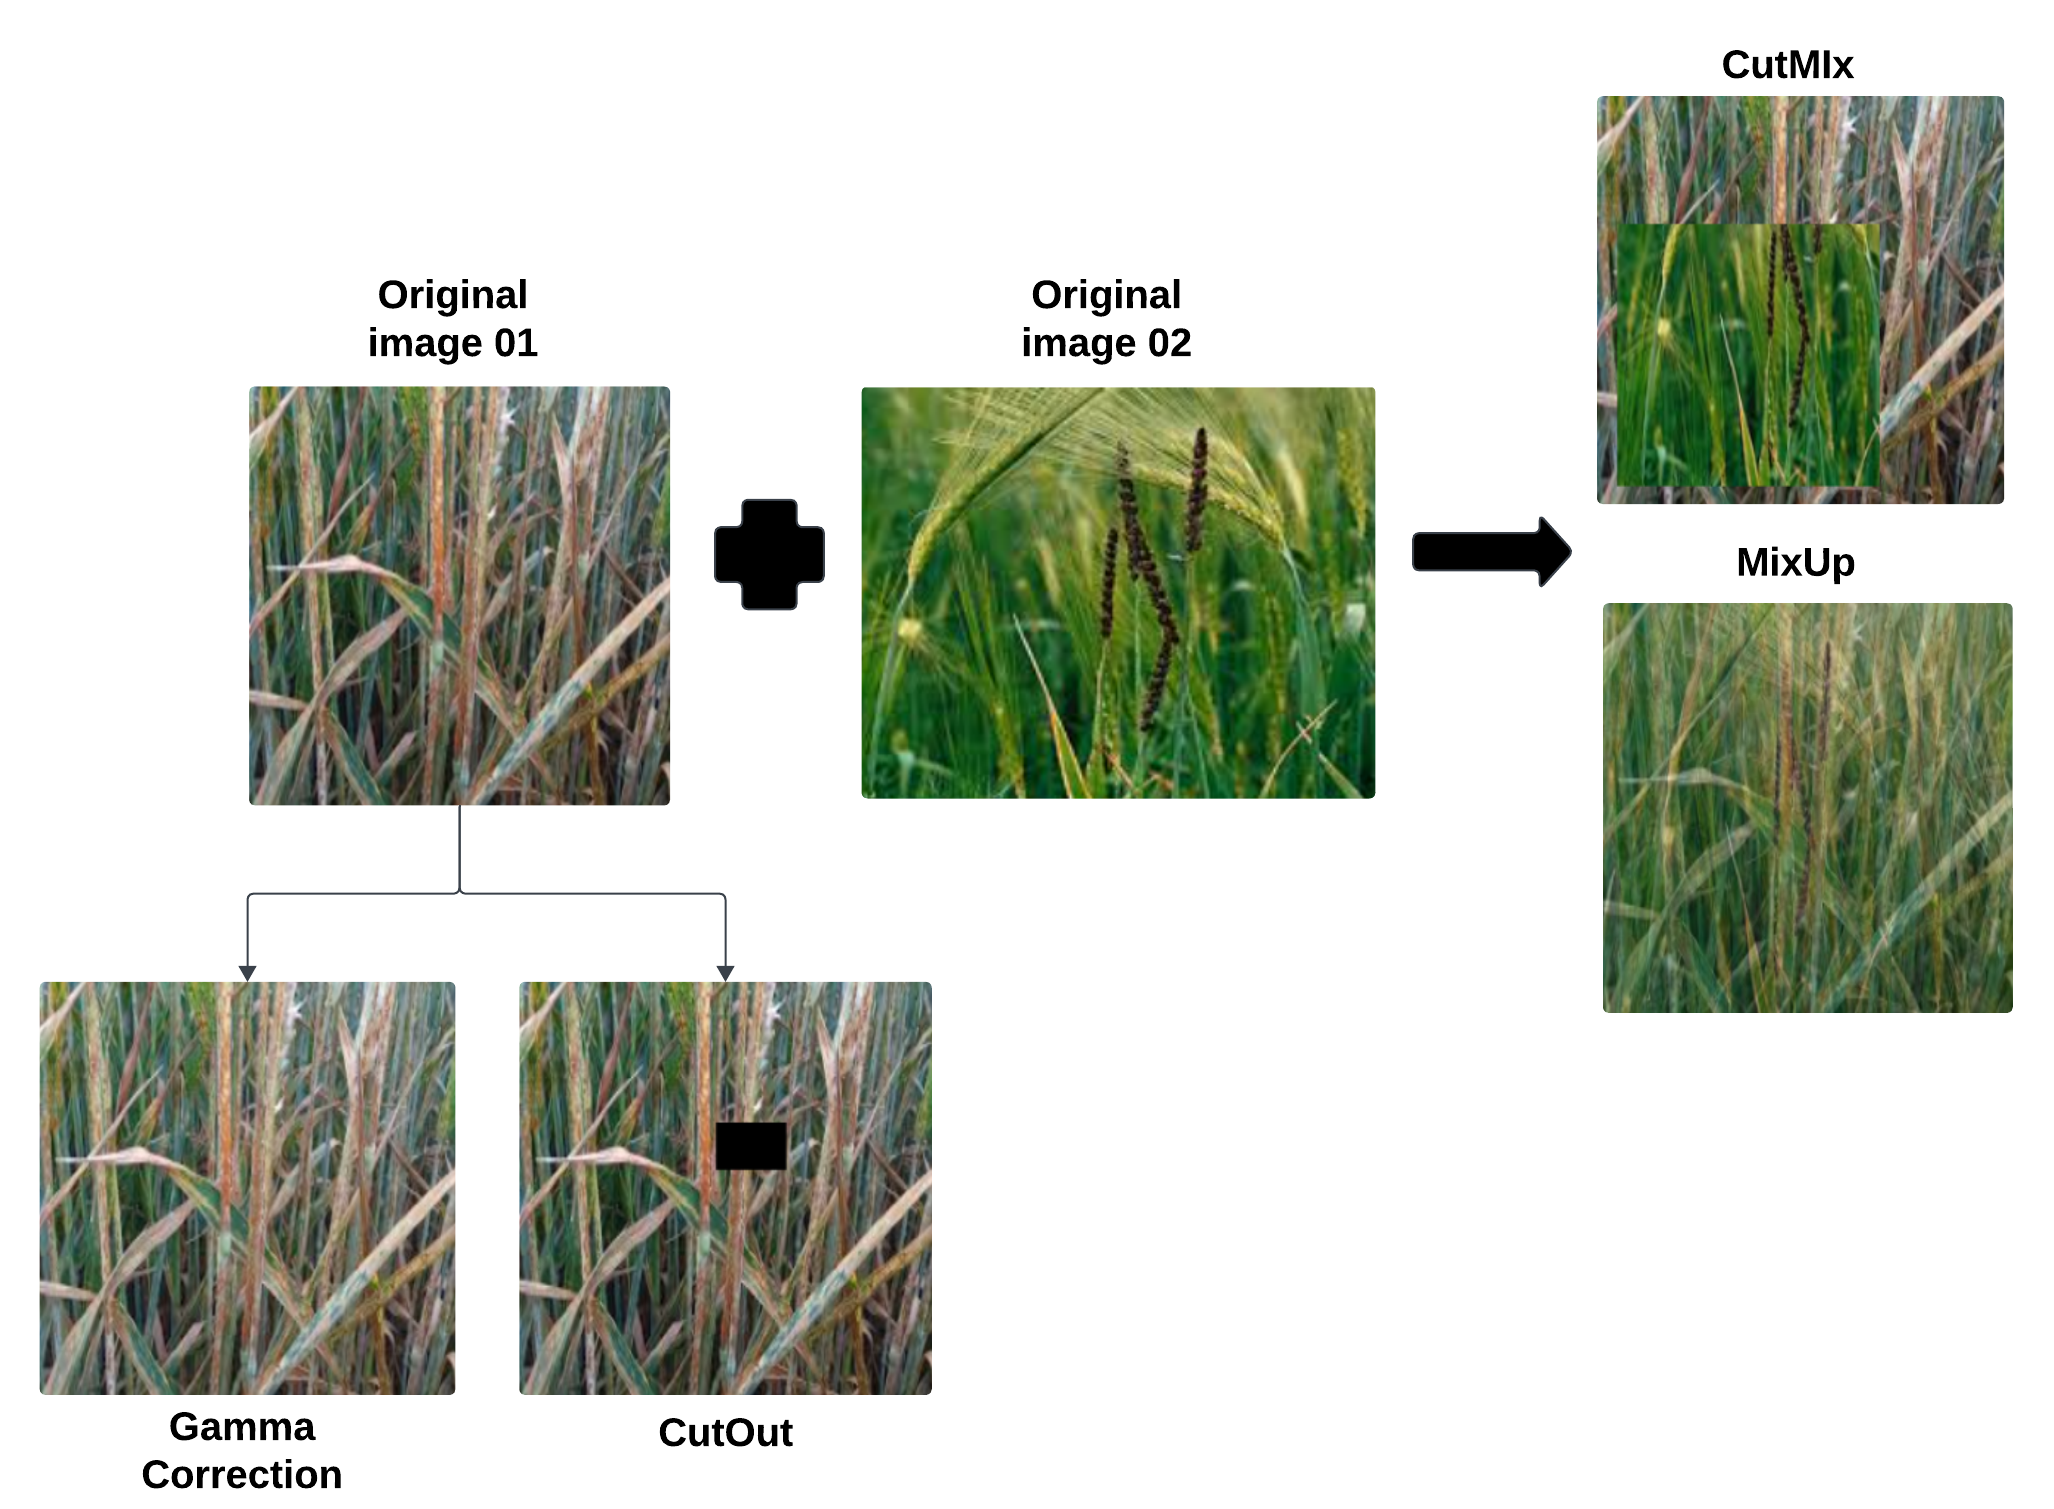
\includegraphics[width=0.7\textwidth]{chapters/chapter5/images/Figure01.png}
    \caption{Data augmentation techniques (Example of application).}
    \label{fig:DataaugmentationExemple}
\end{figure}

Figure~\ref{fig:Model2Dataaugmentation} shows the class distributions after data augmentation. Classes are well balanced, ensuring an equal number of samples for class 0 (Healthy) and class 1 (Not-Healthy), which helps prevent training bias.


\begin{figure}[H] % 'H' needs \usepackage{float}
    \centering
    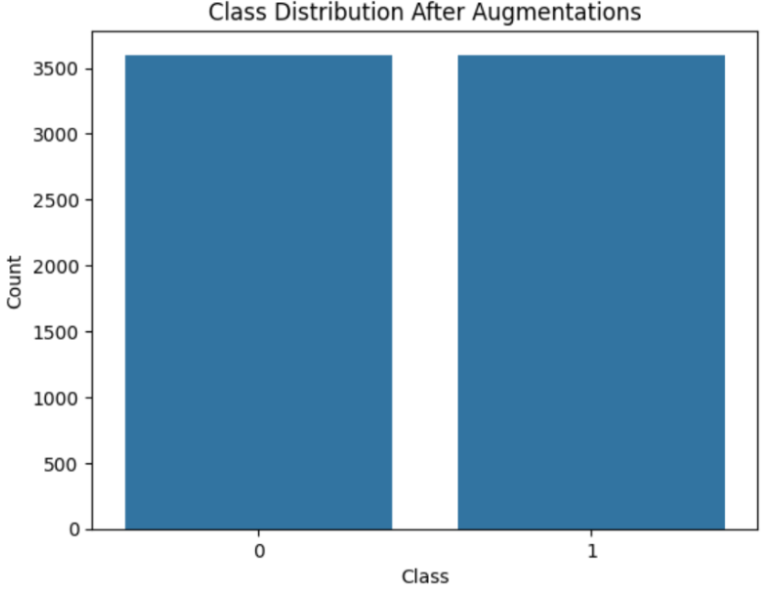
\includegraphics[width=0.7\textwidth]{chapters/chapter5/images/Figure02b.png}
    \caption{Class Distribution After Augmentation..}
    \label{fig:Model2Dataaugmentation}
\end{figure}



\subsubsection{Feature Extraction}
The feature extraction process involves several key steps and configurations:
\begin{itemize}
    \item A batch size of 32 is used throughout the feature extraction process.
    
    \item Feature extraction is performed using EfficientNetB2, VGG19, and DenseNet169, all pre-trained on \textit{ImageNet} for robust initialization and faster convergence.
    
    \item Model adaptation is applied by setting the \texttt{include\_top} parameter to \texttt{false}, which removes the final \textit{ImageNet} classification layers and allows the models to serve as feature extractors for wheat disease classification.
    
    \item After feature extraction, a GlobalAveragePooling2D layer is applied, converting the 3D feature maps (height $\times$ width $\times$ channels) into a 1D feature vector by averaging the values across the spatial dimensions (height and width), thereby reducing dimensionality while preserving the most important features.
\end{itemize}

\subsubsection{Hyperparameter Optimization for Support Vector Machine (SVM) Classifier}

To enhance the predictive performance of the Support Vector Machine (SVM) classifier within the ensemble, a systematic hyperparameter optimization was conducted using \texttt{GridSearchCV}. This approach combines exhaustive grid search, which evaluates all possible combinations of specified hyperparameters, with cross-validation to ensure reliable and unbiased performance estimation. Specifically, 3-fold cross-validation was employed, where the training data is partitioned into three subsets; in each iteration, two subsets are used for training while the remaining one is used for validation. This process is repeated three times, and the performance metrics are averaged to reduce overfitting and ensure the model generalizes well to unseen data.

To improve computational efficiency, parallel processing was enabled by setting \texttt{n\_jobs = -1}, allowing the use of all available CPU cores during the grid search process. Additionally, for scenarios involving class imbalance, the \texttt{class\_weight} parameter was set to \texttt{"balanced"}, automatically adjusting weights inversely proportional to class frequencies in the training set.

Key hyperparameters for the SVM classifier were tuned to identify the optimal configuration, as summarized in Table~\ref{tab:svm_grid}. These include the regularization parameter \texttt{C}, kernel type, kernel coefficient \texttt{gamma}, and polynomial \texttt{degree} (relevant when using a polynomial kernel). These parameters were selected based on their significant impact on the SVM’s decision boundary and generalization ability.

\begin{table}[h]
\centering
\caption{Grid search configuration of SVM classifier hyperparameters}
\begin{tabular}{|p{4.5cm}|p{8.5cm}|}
\hline
\textbf{Hyperparameters} & \textbf{Explored Values} \\
\hline
C (Regularization parameter) & \{0.1, 1, 10\} \\
\hline
Kernel (type of kernel function) & \{linear, rbf, poly\} \\
\hline
gamma (kernel coefficient) & \{scale, auto\} \\
\hline
degree (polynomial degree) & \{2, 3, 4\} \\
\hline
\end{tabular}
\label{tab:svm_grid}
\end{table}

After conducting the grid search with cross-validation, the best-performing configuration for the SVM classifier was identified, as shown in Table~\ref{tab:svm_best}. These hyperparameters were selected based on their cross-validated performance and were used in the final ensemble to ensure optimal and consistent results.

\begin{table}[h]
\centering
\caption{Best hyperparameter settings selected by Grid Search for SVM classifier}
\begin{tabular}{|p{4.5cm}|p{8.5cm}|}
\hline
\textbf{Hyperparameters} & \textbf{Selected Values} \\
\hline
C & 10 \\
\hline
degree & 2 \\
\hline
gamma & scale \\
\hline
kernel & rbf \\
\hline
\end{tabular}
\label{tab:svm_best}
\end{table}




\subsection{Implementation of Multi-Class classification model}
As with the binary classification model, we followed a systematic approach to implement the multi-class classification model. We present the key hyperparameters, data processing strategies, and optimization techniques adapted to handle multiple classes effectively.
\subsubsection{Data preprocessing and data augmentation}
\label{sec:data_augmentation}
The dataset was split into three subsets to ensure robust model training and evaluation: 70\% of the images were allocated for training, 15\% for validation, and 15\% for testing. This stratified split allowed for performance monitoring during training and unbiased assessment on unseen samples.
To enhance the generalization ability of the crop disease classification model, comprehensive data preprocessing and augmentation strategies were employed. This process was implemented using the Albumentations library, integrated through a custom AlbumentationsDataset class that seamlessly applies transformations during data loading. 

The preprocessing pipeline for the training set includes a combination of geometric transformations (resizing, random cropping, rotation, flipping, and shifting), color modifications (brightness, contrast, hue, saturation), and noise simulation (Gaussian blur), followed by normalization and conversion to tensors. For validation and testing, a simplified preprocessing consisting of resizing and normalization was applied to preserve image fidelity. The visual effect of these augmentations is illustrated in Figure~\ref{fig:VisualExamples}, which showcases the diversity of image variations introduced by the pipeline and the exact parameters used in each augmentation technique are detailed in Table~\ref{tab:ImagePreprocessingConfig}, providing a clear summary of the settings chosen for the implementation.

\begin{figure}[H] % 'H' needs \usepackage{float}
    \centering
    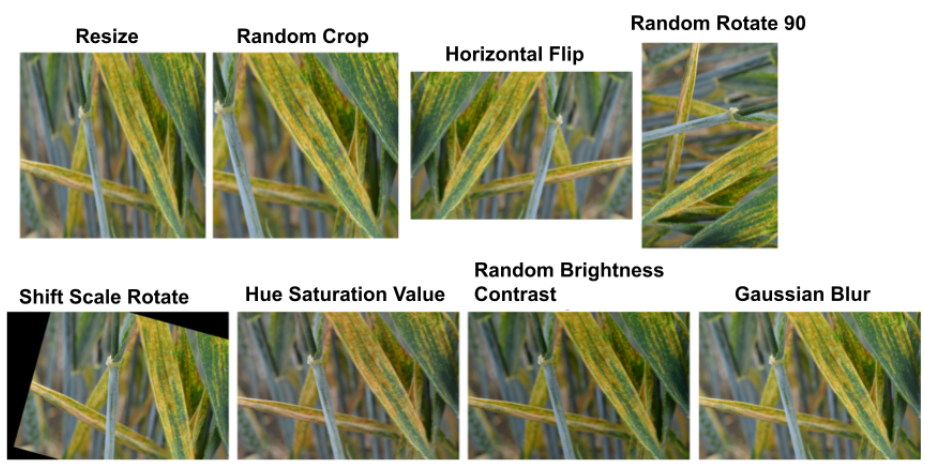
\includegraphics[width=0.9\textwidth]{chapters/chapter5/images/Figure08.png}
    \caption{Visual Examples of Image Variations Generated Through Data Augmentation Techniques.}
    \label{fig:VisualExamples}
\end{figure}


\begin{table}[ht]
\centering
\caption{Configuration of parameters for image preprocessing and augmentation techniques.}
\renewcommand{\arraystretch}{1.3}
\begin{tabular}{|l|p{9cm}|}
\hline
\textbf{Data Processing Technique} & \textbf{Parameter(s) and Value(s)} \\
\hline
Resize & Height: 512, Width: 512 \\
\hline
Random Crop & Height: 448, Width: 448 \\
\hline
Horizontal Flip & Probability: 0.5 \\
\hline
Random 90° Rotation & Probability: 0.5 \\
\hline
Shift, Scale, Rotate & Shift limit: 0.1, Scale limit: 0.1, Rotate limit: 20°, Probability: 0.5 \\
\hline
Hue, Saturation, Value Shift & Hue limit: ±10, Saturation limit: ±15, Value limit: ±10, Probability: 0.5 \\
\hline
Brightness and Contrast & Probability: 0.5 \\
\hline
Gaussian Blur & Blur limit: 3, Probability: 0.3 \\
\hline
Normalize & Mean: (0.485, 0.456, 0.406), Std: (0.229, 0.224, 0.225) \\
\hline
\end{tabular}
\label{tab:ImagePreprocessingConfig}
\end{table}




\subsubsection{Implementation details: Architecture, optimization, and training}
The model architecture is built upon a pretrained ResNet50 from the \texttt{torchvision.models} library, which serves as the backbone for feature extraction. The default fully connected layer is removed and replaced with a custom classification head that integrates an Efficient Channel Attention (ECA) mechanism. This mechanism enables the model to dynamically focus on the most informative regions of the input image, thereby enriching the feature representation with global context. To reduce overfitting, a dropout layer with a rate of 0.3 is applied before the final classification layer, which transforms the 2048-dimensional feature vector into predictions across the eight target classes.

For training, the loss function used is the Cross-Entropy Loss with label smoothing, which mitigates model overconfidence by preventing overly peaked predictions \parencite{szegedy2016rethinking}. The smoothed loss function is defined in equation~\ref{eq:label_smoothing} as a combination of the standard cross-entropy loss (Equation~\ref{eq:cross_entropy}) and a uniform distribution over all $K$ classes::

\begin{equation}
L_{\text{smooth}} = (1 - \varepsilon) \cdot L_{\text{CE}} + \frac{\varepsilon}{K}
\label{eq:label_smoothing}
\end{equation}

\begin{equation}
L_{\text{CE}} = \sum_{i=1}^{K} y_i \log(p_i)
\label{eq:cross_entropy}
\end{equation}

Where:
\begin{itemize}
  \item $K$: Number of classes
  \item $y_i$: 1 if the true class is $i$, otherwise 0
  \item $p_i$: Predicted probability for class $i$
  \item $\varepsilon$: Smoothing factor (0.1)
\end{itemize}


The optimization process relies on Stochastic Gradient Descent (SGD) with momentum and weight decay to train the model efficiently. Unlike standard gradient descent, momentum accumulates a moving average of past gradients to accelerate convergence and reduce oscillations, especially in the presence of high curvature or noisy gradients.

The update rules for SGD with momentum, as described by \parencite{loshchilov2016sgdr}, are given in equation~\ref{eq:sgd_momentum}.

\begin{align}
v_{t+1} &= \mu v_t + \eta \nabla w_t \\
w_{t+1} &= w_t - v_{t+1}
\label{eq:sgd_momentum}
\end{align}




Where:  
\begin{itemize}
  \item $v_t$: velocity (momentum term)
  \item $\mu$: momentum coefficient (set to 0.9)
  \item $\eta$: learning rate (initially 0.001)
  \item $\nabla w_t$: gradient of the loss with respect to the parameters $w$
\end{itemize}

To mitigate overfitting, weight decay (L2 regularization) is applied with a coefficient set to $10^{-5}$ to penalize large weights and promote simpler, more generalizable models.

Instead of maintaining a constant learning rate throughout training, a cosine annealing schedule is employed to adjust it dynamically. This schedule starts with larger learning rates to allow broader exploration of the loss landscape and gradually reduces them to smaller steps as training progresses, enabling precise fine-tuning near the optimum. The cosine shape of the decay curve ensures a smooth transition between exploration and exploitation phases, facilitating stable and efficient convergence.

The learning rate $\eta_t$ at epoch $t$ is given by equation~\ref{eq:cosine_lr} \parencite{loshchilov2016sgdr}.

\begin{equation}
\eta_t = \eta_{\min} + \frac{1}{2}(\eta_{\max} - \eta_{\min}) \left(1 + \cos\left(\frac{t}{T} \pi\right)\right)
\label{eq:cosine_lr}
\end{equation}



Where:  
\begin{itemize}
  \item $\eta_{\max}$: initial learning rate (0.001)
  \item $\eta_{\min}$: minimum learning rate (typically $10^{-5}$)
  \item $T$: total number of epochs ($T = 25$)
\end{itemize}

The model was trained for 25 epochs with a batch size of 16. Weighted Random Sampling was applied to handle class imbalance during training by assigning a higher sampling probability to under-represented classes.

Figure~\ref{fig:Model3TrainingPerformance} below summarizes the learning behavior of the model:
\begin{itemize}
    \item \textbf{Loss Curves:} A consistent decrease in both training and validation losses over epochs, indicating proper fitting.
    \item \textbf{Accuracy Curves:} A steady increase reaching high accuracy on both training and validation sets, without significant divergence, suggesting that the model generalizes well without overfitting.
\end{itemize}

\begin{figure}[H] % 'H' needs \usepackage{float}
    \centering
    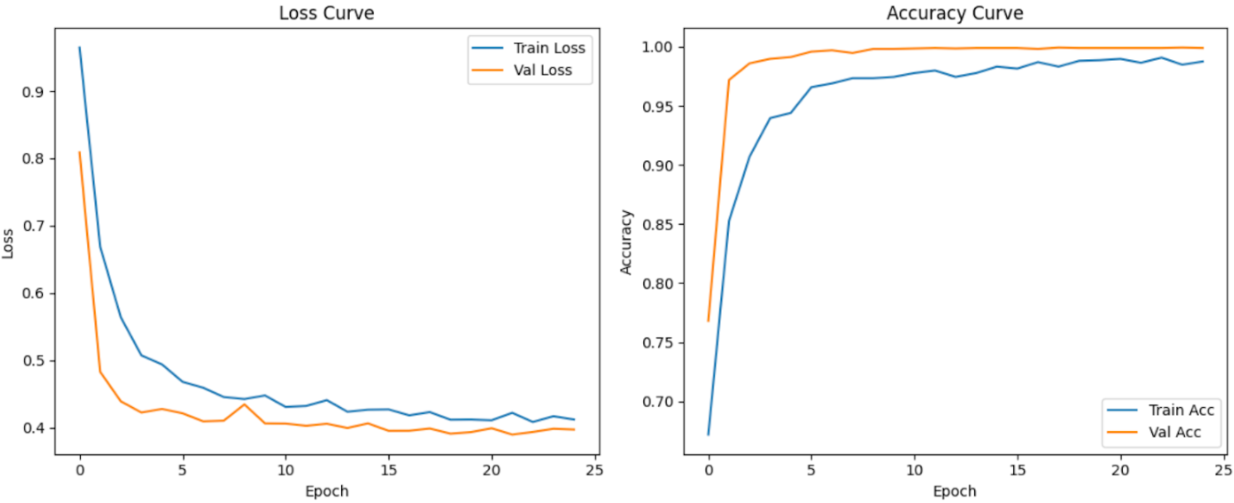
\includegraphics[width=0.9\textwidth]{chapters/chapter5/images/Figure03.png}
    \caption{Model 3 Training Performance: Loss and Accuracy Curves.}
    \label{fig:Model3TrainingPerformance}
\end{figure}

\section{Implementation of the Wheat Insect Pest Detection Model}

The insect pest detection task required a shift toward object detection techniques capable of identifying and localizing pests in wheat field images. This was achieved using the YOLOv8 architecture, particularly its oriented bounding box (OBB) variant, which is well-suited for detecting small and variably-angled objects as presented before in the solution design chapter.

\subsubsection{Data preparation and annotation}

The original dataset consisted of high-resolution field images containing visible pest instances. Each image was manually annotated using the cvat tool (Computer Vision Annotation Tool), with annotations exported in the Ultralytics YOLO Oriented Bounding Boxes 1.0 format. These annotations define the object class along with eight floating-point numbers representing the rotated bounding box coordinates.

The dataset was then split into training and testing sets using an 80/20 ratio. A Python script was developed to automate this split and organize the data into the appropriate folder structure required by the YOLO framework. The distribution of samples in each subset is presented in Table~\ref{tab:split}.

\begin{table}[h]
\centering
\caption{Dataset split summary}
\begin{tabular}{|c|c|c|}
\hline
\textbf{Subset} & \textbf{Number of Images} & \textbf{Number of Annotations} \\
\hline
Training & 1346 & 3315 \\
Testing & 345 & 481 \\
\hline
\textbf{Total} & \textbf{1691} & \textbf{3796} \\
\hline
\end{tabular}
\label{tab:split}
\end{table}



To ensure consistency and avoid training errors, a preprocessing step was performed to verify the integrity of label files. This included:
\begin{itemize}
    \item Removing malformed entries with incorrect coordinate counts.
    \item Clipping coordinates to ensure they remain within the normalized \([0,1]\) range.
    \item Formatting labels to maintain precision and consistency across the dataset.
\end{itemize}

\subsubsection{Data augmentation techniques}

To improve the generalization ability of the model and enhance robustness to various field conditions, several data augmentation techniques were applied during training. These augmentations were particularly important for detecting small and variably-oriented objects in cluttered environments. The applied augmentations and their corresponding configurations are listed in Table~\ref{tab:augmentations}.

\begin{table}[H]
\centering
\caption{Data augmentation parameters}
\label{tab:augmentations}
\begin{tabular}{|c|c|}
\hline
\textbf{Augmentation Technique} & \textbf{Value} \\
\hline
Image Rotation (\texttt{degrees}) & 45° \\
Horizontal Flip Probability (\texttt{fliplr}) & 0.5 \\
Vertical Flip Probability (\texttt{flipud}) & 0.5 \\
MixUp (\texttt{mixup}) & 0.2 \\
Copy-Paste (\texttt{copy\_paste}) & 0.2 \\
Hue Variation (\texttt{hsv\_h}) & 0.015 \\
Saturation Variation (\texttt{hsv\_s}) & 0.7 \\
Brightness Variation (\texttt{hsv\_v}) & 0.4 \\
\hline
\end{tabular}
\end{table}

\subsubsection{Model Selection and Training Configuration}

For this task, the YOLOv8m-OBB model provided by Ultralytics was selected due to its balance between accuracy and computational efficiency. The training process was configured using parameters that ensure optimal convergence while maintaining a reasonable computational load. Table~\ref{tab:train-config} summarizes the key settings used throughout training.

\begin{table}[H]
\centering
\caption{YOLOv8m-OBB Training Configuration}
\label{tab:train-config}
\begin{tabular}{|c|c|}
\hline
\textbf{Parameter} & \textbf{Value} \\
\hline
Model & YOLOv8m-OBB \\
Epochs & 300 \\
Batch Size & 16 \\
Image Size & 640 × 640 \\
Optimizer & AdamW \\
Initial Learning Rate (\texttt{lr0}) & 0.001 \\
Learning Rate Factor (\texttt{lrf}) & 0.01 \\
Weight Decay & 0.0005 \\
Patience & 50 \\
Number of Workers & 4 \\
Objectness Weight (\texttt{kobj}) & 2.0 \\
\hline
\end{tabular}
\end{table}



\section{Implementation of the AI Assistant}

This AI assistant is powered by Google's Gemini API and allows users to input questions or photos of wheat crops to receive real-time AI-generated feedback.The assistant was implemented as a web API using the Flask microframework.The entire process from user input to response generation and return is visually summarized in Figure~\ref{fig:chatbot-process}. The main components are described below:

\begin{itemize}
    \item \textbf{API access key acquisition:}  
    An API key was obtained from the Google AI Studio platform, which grants access to the Gemini models via the \texttt{google.generativeai} Python package.

    \item \textbf{Environment variable configuration:}  
    To secure the API key and prevent hardcoding, it was stored in an \texttt{.env} file. This variable is loaded securely during runtime to configure the Gemini SDK.

    \item \textbf{Setting up Flask with CORS:}  
    A Flask server was initialized to handle HTTP requests. CORS (Cross-Origin Resource Sharing) was enabled to allow access from front-end applications hosted on different domains.

    \item \textbf{Gemini Flash model integration:}  
    The \texttt{gemini-1.5-flash} model was selected due to its efficiency and support for both image and text inputs. The model was initialized once using the configured API key.

    \item \textbf{Handling chat requests:}  
    The endpoint \texttt{/chatbot} listens for POST requests containing either a textual message, an image, or both. Submitted images are validated for allowed file types and verified to ensure they are readable.

    \item \textbf{Sending requests to Gemini:}  
    If the input is valid, the message and/or image are appended to a content list and sent to the Gemini model using the \texttt{generate\_content} method. The response is then extracted and returned to the front end in JSON format.

    \item \textbf{Error handling:}  
    Proper exception handling is implemented to catch unexpected runtime issues and return appropriate error messages to the client, while logging them on the server.
\end{itemize}



\begin{figure}[H]
\centering
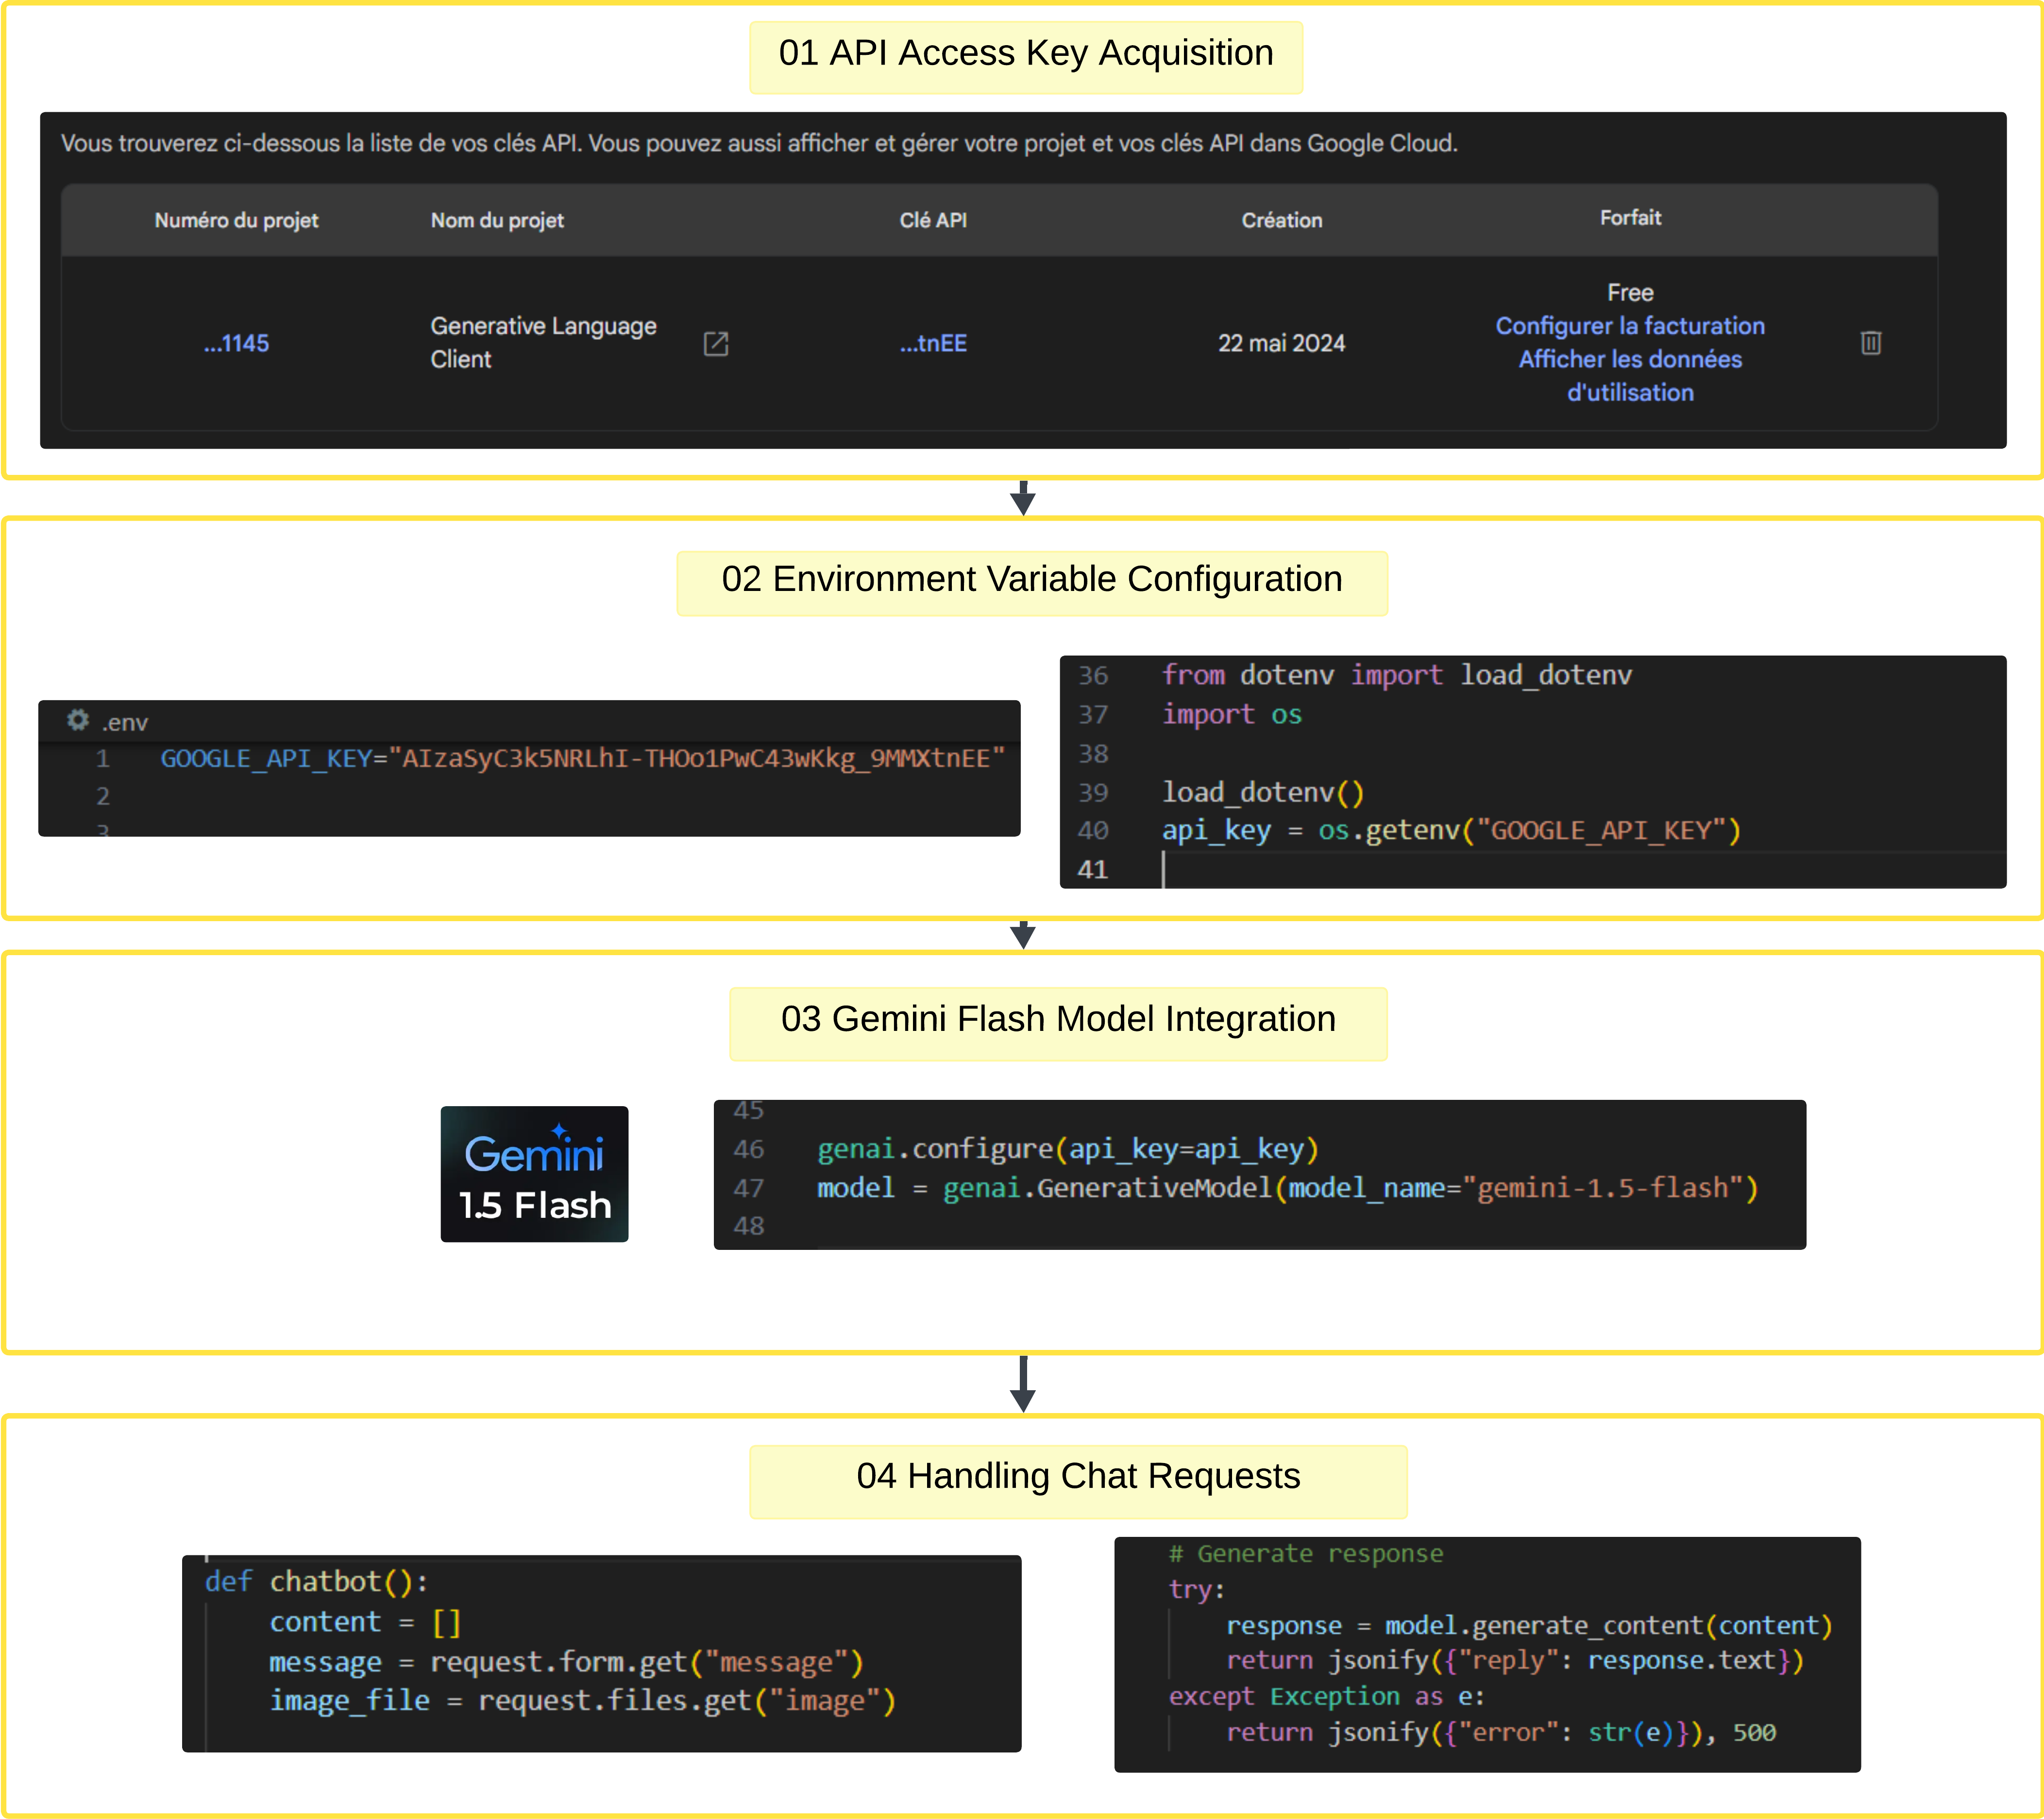
\includegraphics[width=1\textwidth]{chapters/chapter5/images/Figure13.png}
\caption{Pipeline of the AI assistant from input reception to Gemini-based response generation.}
\label{fig:chatbot-process}
\end{figure}



\section{Implementation of the web platform}
The deployment of the trained models was carried out through the Wheat Guard web platform, enabling real-time interaction with users. The platform also features intuitive interfaces that support image uploads, disease classification, and pest detection functionalities.
\subsection{Model integration}
In machine learning and deep learning workflows, saving trained models is a key step, whether for future inference, continued fine-tuning, or deployment. The choice of file format depends on the framework used and the intended purpose. Gaining a solid understanding of these formats ensures efficient model management and smooth transitions throughout the development pipeline.

\begin{itemize}
    \item \textbf{.pkl}: Commonly used with traditional machine learning libraries like \texttt{scikit-learn}, this format stores complete Python objects, including trained models, using Python’s \texttt{Pickle} serialization protocol.

    \item \textbf{.pth / .pt}: These formats are native to \texttt{PyTorch}. They are used to save model weights or full models. While functionally similar, \texttt{.pt} is generally preferred for deployment, especially when models are exported with \texttt{TorchScript}.

    \item \textbf{.h5}: Used by \texttt{Keras} and \texttt{TensorFlow}, this format (based on the \texttt{HDF5} standard) stores both the model architecture and its trained weights, making it ideal for saving and later reconstructing a complete model.
\end{itemize}

Table~\ref{tab:ModelSaveFormats} provides an overview of the save formats used in the Smart Wheat Monitoring System. Each model was saved using the format recommended by its respective implementation framework.

\begin{table}[H]
\centering
\renewcommand{\arraystretch}{1.3}
\caption{Summary of model save formats for the smart wheat monitoring system.}
\begin{tabular}{|l|c|p{7cm}|}
\hline
\textbf{Model} & \textbf{Model Saving Format} & \textbf{Justification} \\
\hline
Model01\_Binary classification & \texttt{.pkl} & Model implemented with scikit-learn \\
\hline
Model02\_Multiclass classification & \texttt{.pth} & The implementation framework is PyTorch \\
\hline
Insect\_pest\_detection & \texttt{.pt} & Waiting for this \\
\hline
\end{tabular}
\label{tab:ModelSaveFormats}
\end{table}


\subsection{Project structure}
The project is structured into two main parts: Frontend and Backend. The Frontend handles the user interface, while the Backend is responsible for model integration, file handling, and API communication.

\begin{figure}[H]
    \centering
    \begin{minipage}{0.55\textwidth}
        \raggedright
        \textbf{The Backend includes:}
        \begin{itemize}
            \item \textbf{app.py}: The entry point of the backend server.
            \item \textbf{config.py}: Contains configuration settings for the application.
            \item \textbf{requirements.txt}: Specifies the Python dependencies.
            \item \textbf{routes/}: Defines \gls{abb:api} endpoints.
            \item \textbf{saved\_models/}: Stores trained \gls{abb:ml} models.
            \item \textbf{uploads/}: Used to store user-uploaded files temporarily.
            \item \textbf{use\_models/}: Includes scripts to load and run predictions using the models.
            \item \textbf{venv/}: The Python \gls{abb:venv} for package isolation.
        \end{itemize}
    \end{minipage}%
    \hfill
    \begin{minipage}{0.4\textwidth}
        \centering
        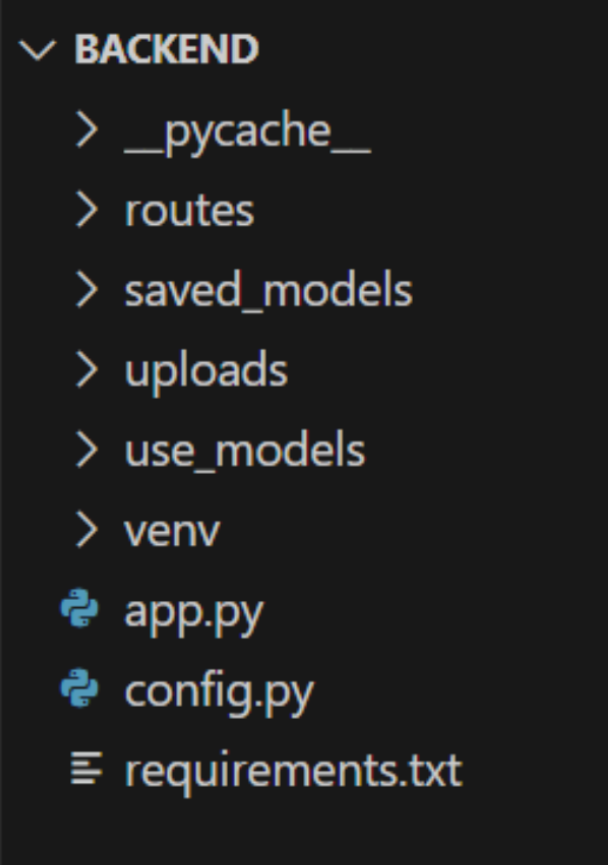
\includegraphics[width=0.9\linewidth]{chapters/chapter5/images/Figure04.png}
        \captionof{figure}{Backend project directory structure.}
        \label{fig:BackendProject}
    \end{minipage}
\end{figure}


\begin{figure}[H]
    \centering
    \begin{minipage}{0.55\textwidth}
        \raggedright
        \textbf{The Frontend includes:}
        \begin{itemize}
            \item \textbf{src/}: Contains all source code for the React application.
            \begin{itemize}
                \item \textbf{assets/}: Directory for static assets such as images or icons.
                \item \textbf{components/}: Contains reusable \gls{abb:ui} components.
                \item \textbf{pages/}: Holds different pages/screens of the application.
                \item \textbf{App.tsx}: Root component that sets up routing and layout.
                \item \textbf{index.css}: Global \gls{abb:css} styles.
                \item \textbf{main.tsx}: Entry point that mounts the React app to the \gls{abb:dom}.
                \item \textbf{vite-env.d.ts}: Type declaration file for Vite.
            \end{itemize}
            \item \textbf{index.html}: Main \gls{abb:html} file used by Vite to render the app.
            \item \textbf{tailwind.config.js}: Tailwind \gls{abb:css} configuration.
            \item \textbf{postcss.config.js}: Configuration for Post\gls{abb:css}.
            \item \textbf{tsconfig.json / tsconfig.node.json}: \gls{abb:ts} compiler settings.
            \item \textbf{vite.config.ts}: Configuration file for the Vite build tool.
            \item \textbf{package.json / package-lock.json}: Manage project dependencies and scripts.
            \item \textbf{.eslintrc.cjs}: ESLint configuration for code quality.
        \end{itemize}
    \end{minipage}%
    \hfill
    \begin{minipage}{0.4\textwidth}
        \centering
        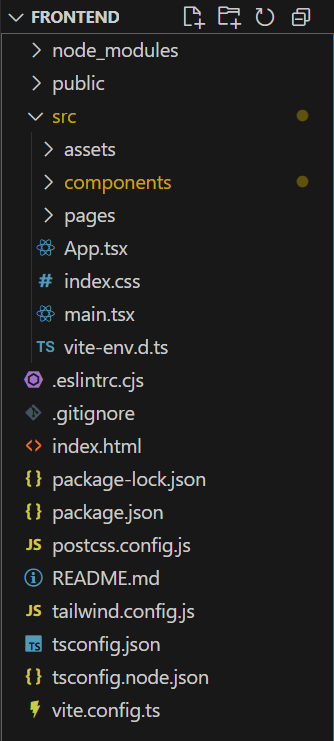
\includegraphics[width=0.9\linewidth]{chapters/chapter5/images/Figure10.png}
        \captionof{figure}{Frontend Project Directory Structure.}
        \label{fig:FrontendProject}
    \end{minipage}
\end{figure}



\subsection{Web platform interfaces}

This section presents the main interfaces of our web application, Wheat Guard, where the models for wheat disease classification and insect pest detection are deployed. Additional interfaces are provided in Appendix\ref{app:annexC}.

\subsubsection{Wheat Disease Detection Interface}
The Wheat Disease Detection Interface (Figure~\ref{fig:uploadImage}) allows users to submit images of wheat crops, perform automated disease detection using trained models, and view classification results with confidence scores. It also highlights infected regions for clearer interpretation (Figure~\ref{fig:WheatDiseaseClassificationpage}).

\begin{figure}[H]
    \centering
    \begin{minipage}{0.48\textwidth}
        \centering
        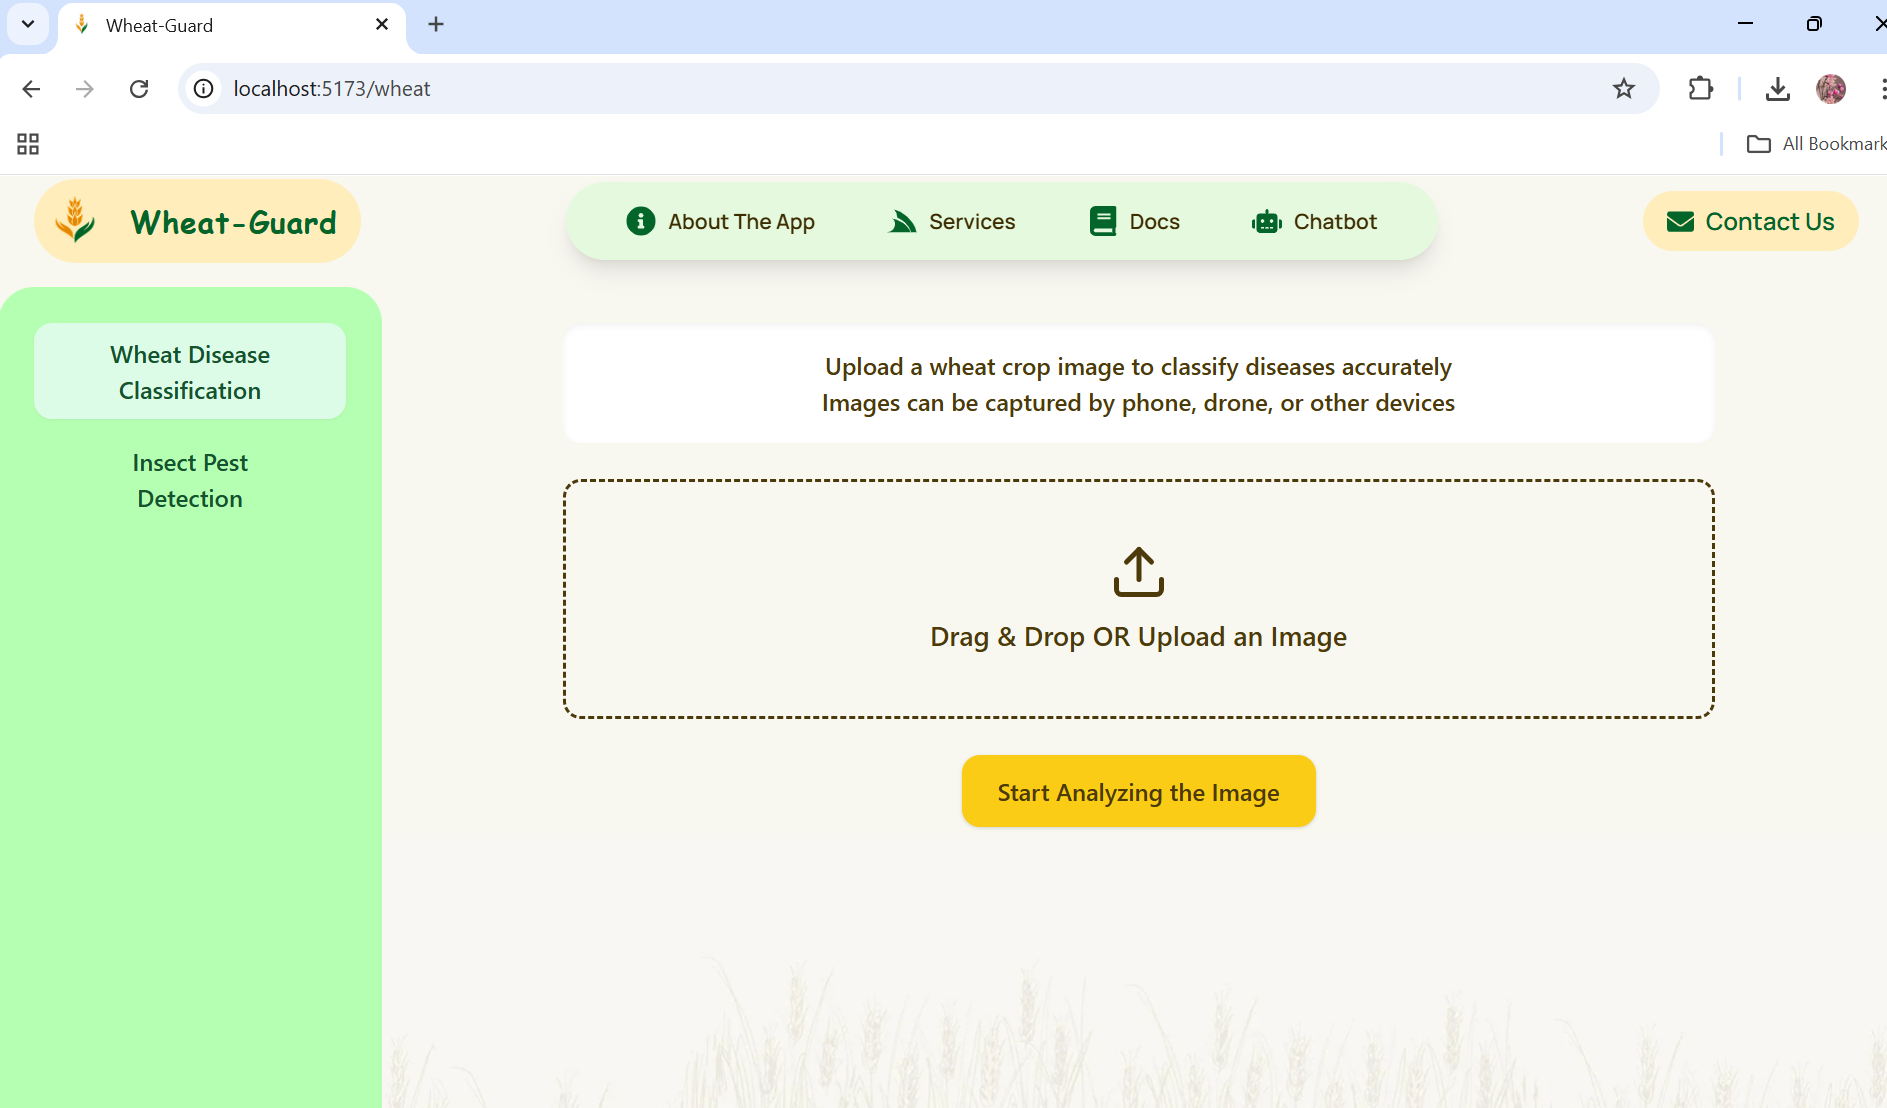
\includegraphics[width=\textwidth]{chapters/chapter5/images/Figure05.png}
        \caption{Upload an image to analyze and detect wheat diseases.}
        \label{fig:uploadImage}
    \end{minipage}
    \hfill
    \begin{minipage}{0.48\textwidth}
        \centering
        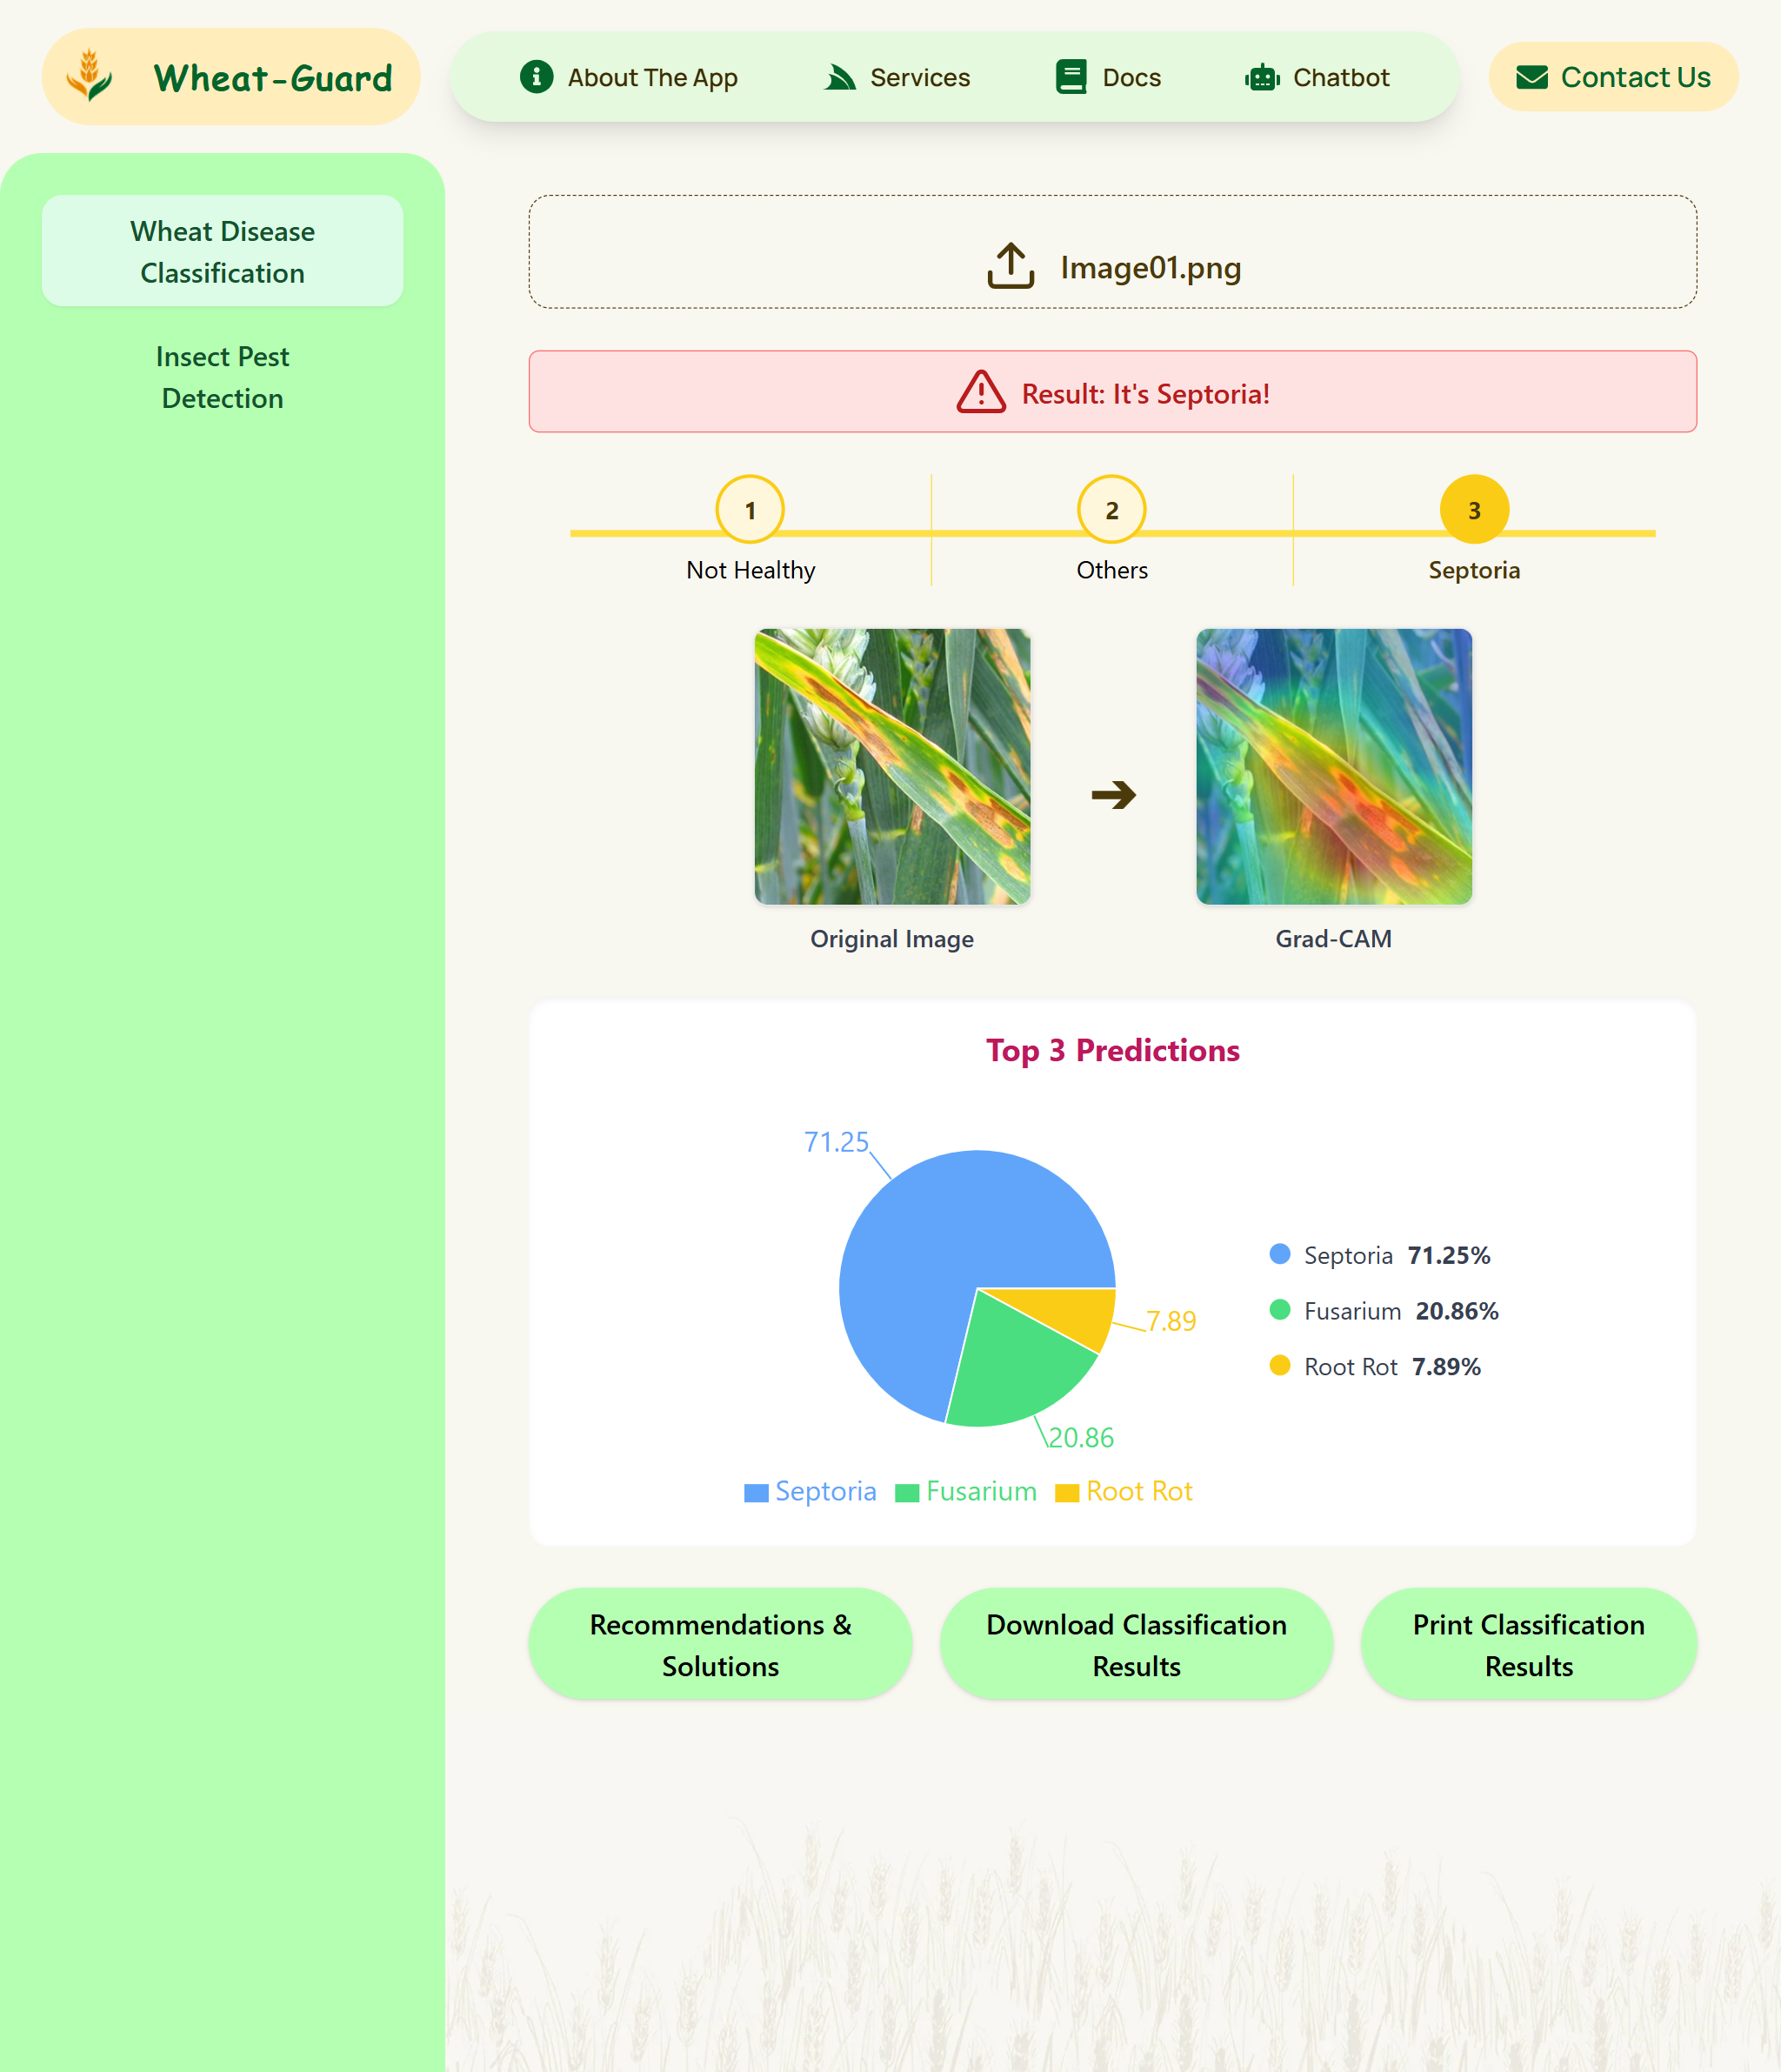
\includegraphics[width=\textwidth]{chapters/chapter5/images/Figure06.png}
        \caption{Wheat disease classification results.}
        \label{fig:WheatDiseaseClassificationpage}
    \end{minipage}
\end{figure}



\subsubsection{Insect pest detection page}

The Insect Pest Detection page (Figure~\ref{fig:Insectpestdetectionpage}) allows users to upload images of wheat crops suspected of pest infestation. The system automatically analyzes the images to identify common insect pests that affect wheat. Users receive detailed detection results along with visual indicators highlighting the regions where pests are detected.

\begin{figure}[H] % 'H' needs \usepackage{float}
    \centering
    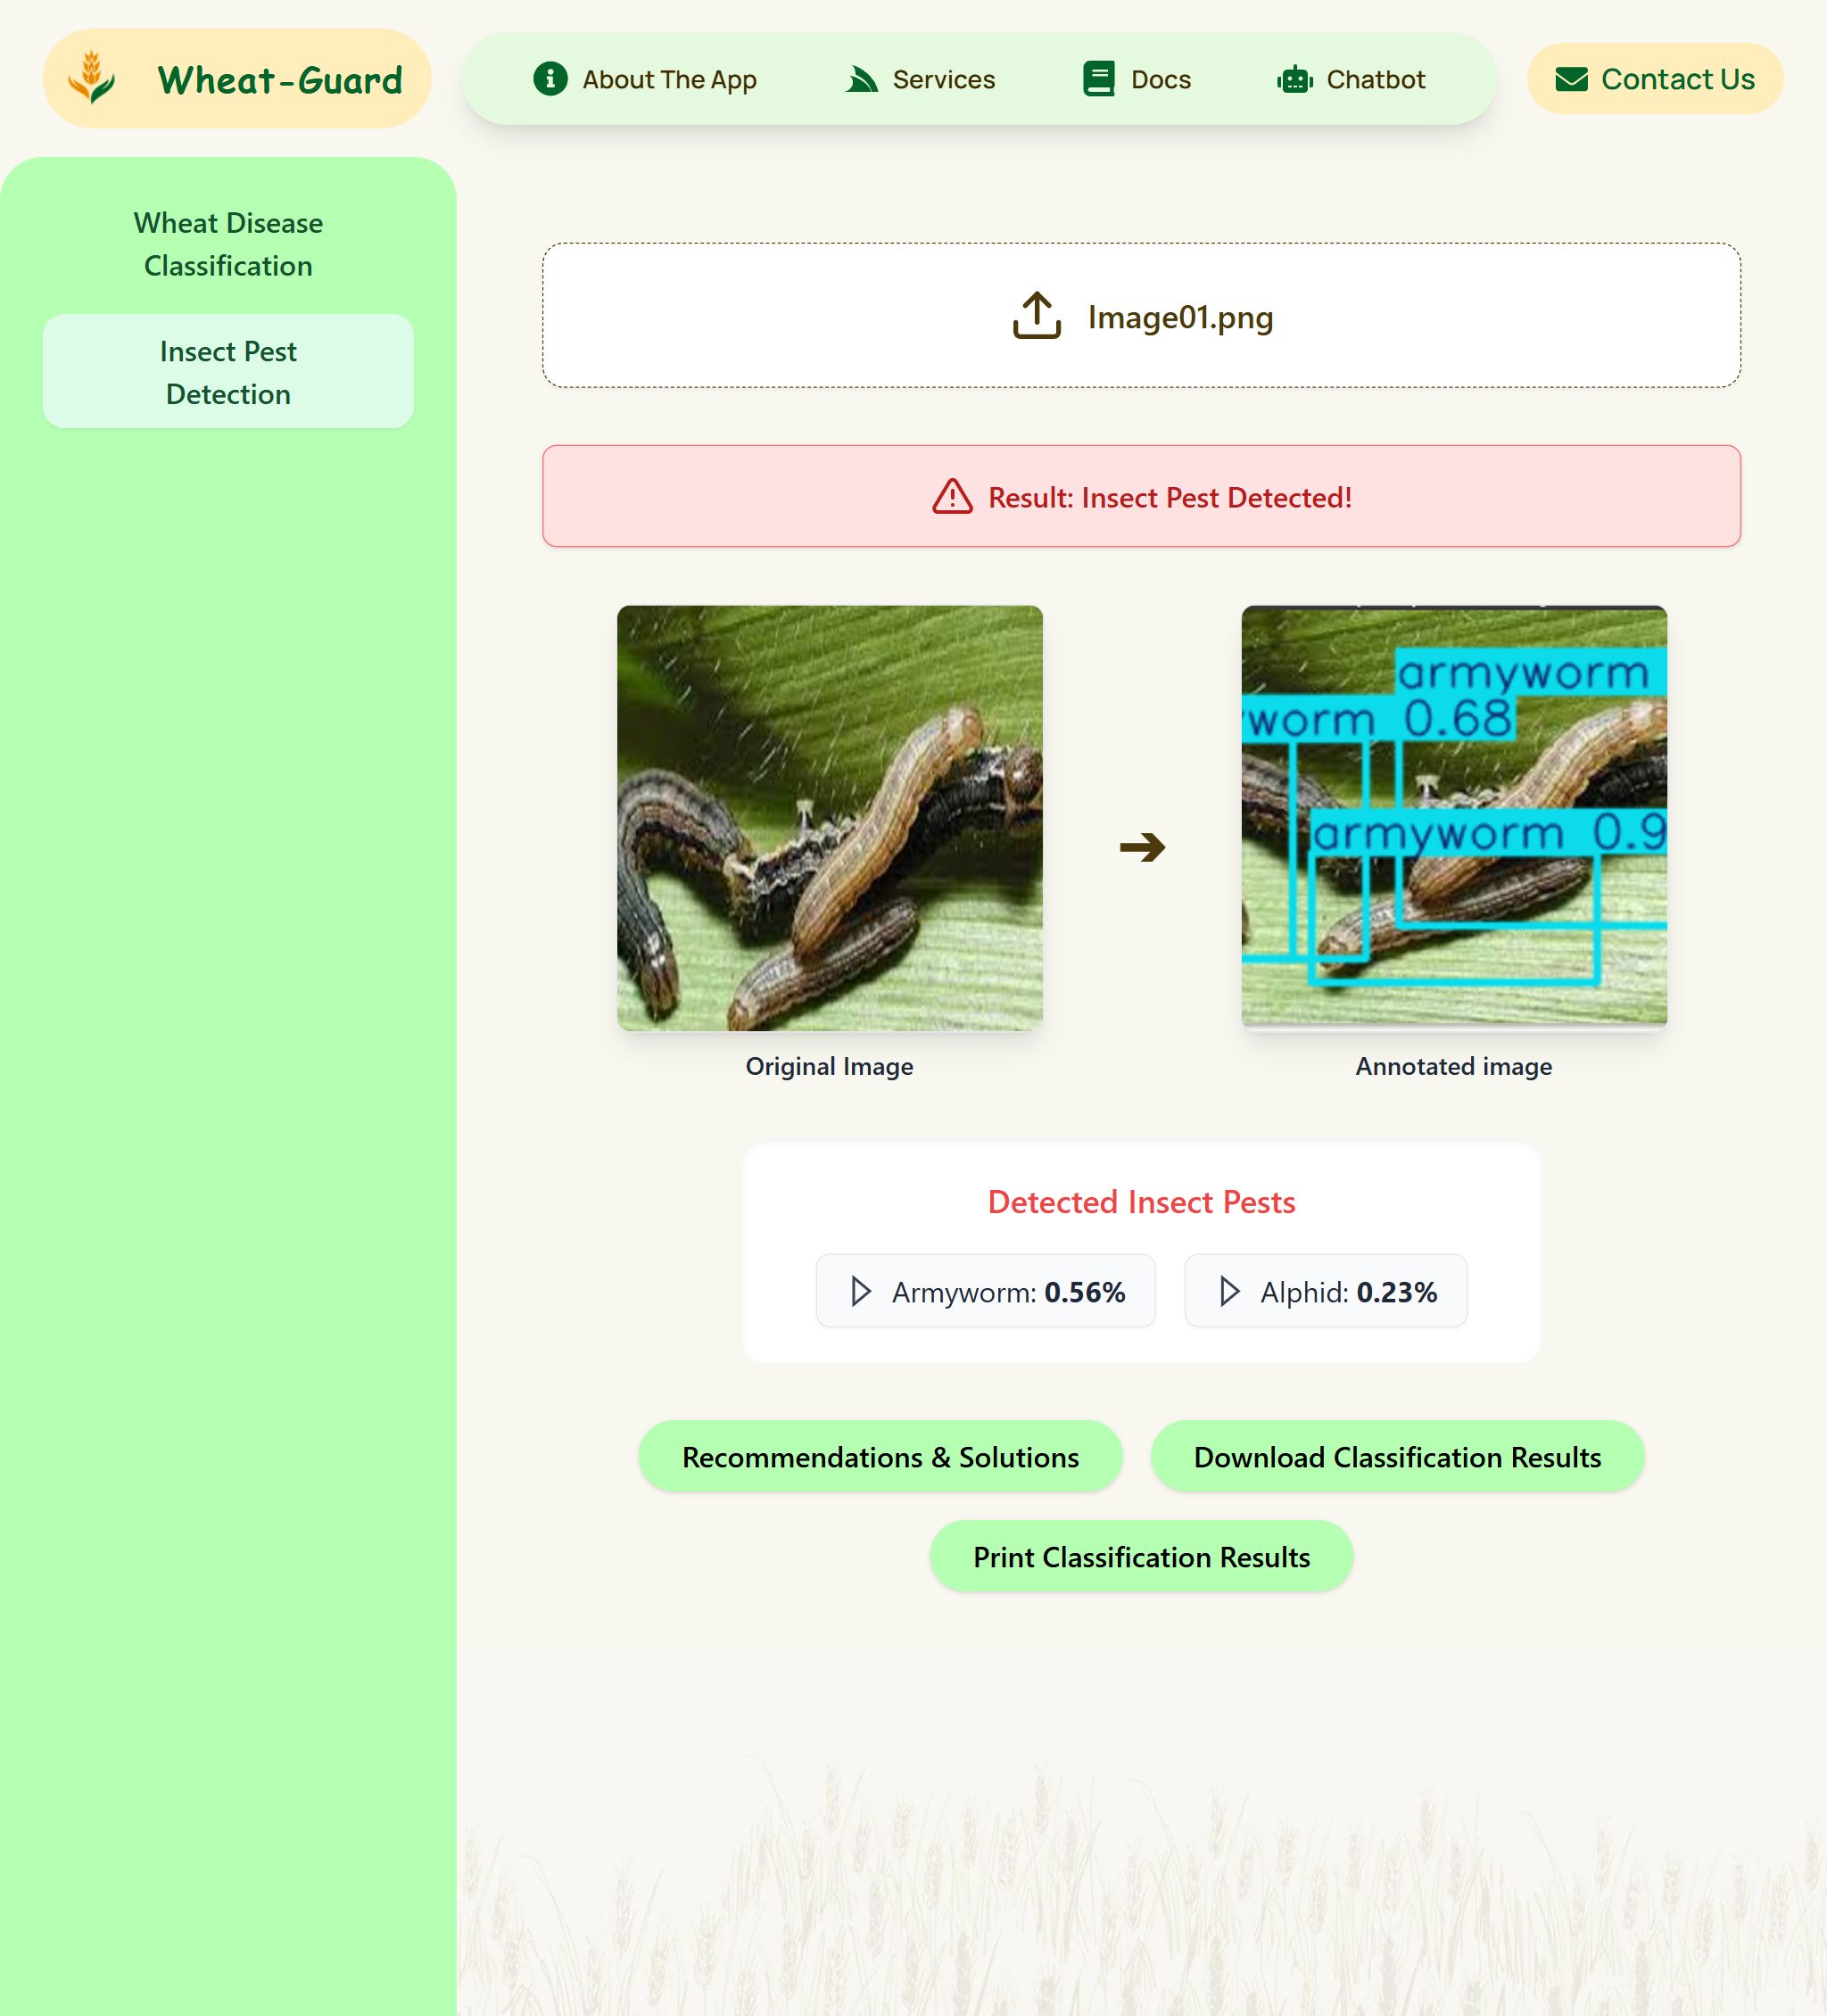
\includegraphics[width=0.7\textwidth]{chapters/chapter5/images/Figure07.png}
    \caption{Insect pest detection page.}
    \label{fig:Insectpestdetectionpage}
\end{figure}


\subsubsection{AI Assistant Page}

The AI Assistant page (Figure~\ref{fig:AIAssistantPage}) is designed to provide users with a conversational interface for interactive support. Users can either send a message or upload an image to ask questions related to wheat diseases and pest control. The assistant leverages an integrated natural language processing model to deliver informative and context-aware responses, making the platform more accessible and user-friendly, especially for non-experts in agriculture or technology.

\begin{figure}[H] % 'H' needs \usepackage{float}
    \centering
    
\includegraphics[width=0.8\textwidth]{chapters/chapter5/images/Figure11.png}
    \caption{AI Assistant page interface.}
    \label{fig:AIAssistantPage}
\end{figure}


\section{Conclusion}
This chapter outlined the complete implementation process of our smart wheat monitoring system, from selecting the appropriate tools to developing and integrating the core modules. With all components successfully implemented and deployed, the next chapter focuses on evaluating their performance through rigorous testing and validation.